\chapter{WKB 近似}
\label{chap:wkb}
\index{WKB 近似}

\section{引言}
\label{sec:wkb-introduction}

WKB 方法以 Gregor Wentzel、Hendrik Kramers 与 Léon Brillouin 的名字命名,用于近似一维 Hamilton 算子的特征函数与特征值.最适合理解这一近似的方式,是在 $\hbar\to0$ 时固定一段能量范围(在许多情形中,也可把它理解为固定 $\hbar$ 而令能量趋于无穷).

WKB 方法的思想是把势函数 $V(x)$ 看作“缓慢变化”的函数,于是定态 Schrödinger 方程的解在局部看起来像常势情形的解.在经典允许区间内,这会产生一个快速振荡的复指数乘以缓慢变化的振幅;指数的局部频率取为常势情形的局部频率.振幅一旦如此选定,就有唯一选择使误差为 $O(\hbar^2)$,但该振幅在转向点(经典粒子改变运动方向的点)附近发散.在经典禁阻区间内,得到的是快速增长或衰减指数乘以缓慢变化因子的近似解,同样在转向点发散.

转向点附近的困难意味着不能像第 5 章那样直接把不同区域的近似解“接起来”.我们将使用 Airy 函数近似转向点附近的 Schrödinger 方程;Airy 函数的渐近式会给出正确的连接条件,它是“旧量子理论”中 Bohr--Sommerfeld 规则的修正版.

\section{旧量子理论与 Bohr--Sommerfeld 条件}
\label{sec:wkb-bohr-sommerfeld}

为简单起见,考虑一个自由度的粒子.令 $C$ 是相空间中 Hamilton 函数的能级集
\[
C=\{(x,p)\in\mathbb R^2\mid H(x,p)=E\},
\label{eq:wkb-energy-curve}
\]
并假设 $C$ 是闭曲线.想象在 $C$ 上画一个“波”,即定义在 $C$ 上的某个振荡函数.按照 de Broglie 假设(见第~\ref{subsec:bohr-debroglie} 节),波的局部频率 $k$(作为 $x$ 的函数)为 $p/\hbar$;所以波的相位应由沿曲线积分 $p\,dx/\hbar$ 得到.波可以写成
\[
\cos\left(\frac1\hbar\int_{x_0}^{x}p\,dx-\delta\right),
\label{eq:wkb-old-wave}
\]
其中 $x_0$ 是曲线上任意起点,$\delta$ 是任意相位.旧量子理论没有给这个波物理解释,它只是试图把波引入图景的一种粗略方法.

\begin{figure}[htbp]
\centering
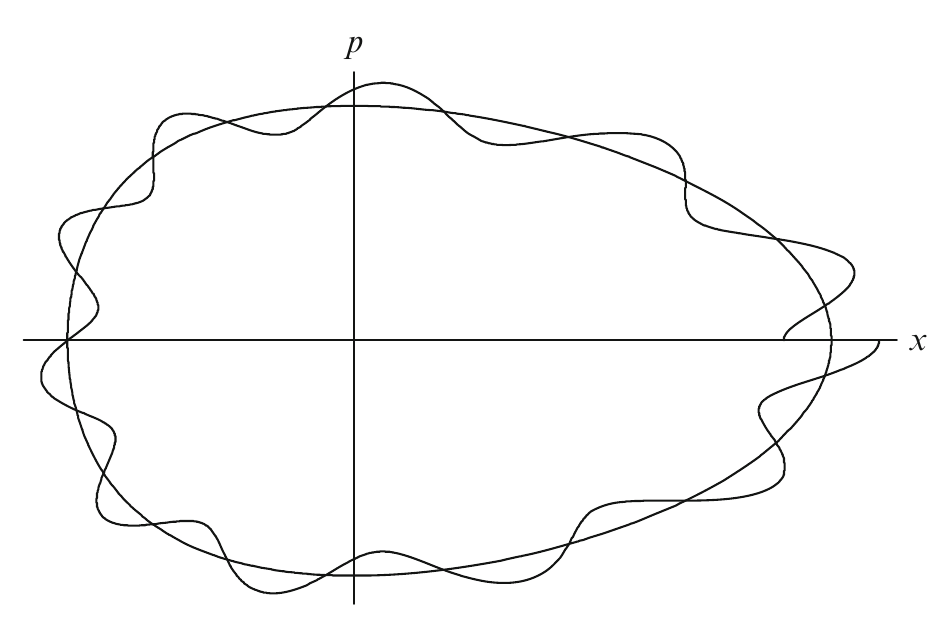
\includegraphics[width=0.76\textwidth]{figures/figure-15-1.png}
\caption{满足修正 Bohr--Sommerfeld 条件的轨道($n=10$).}
\label{fig:wkb-bohr-sommerfeld-trajectory}
\end{figure}

Bohr--Sommerfeld 条件要求沿曲线走一周后式~\eqref{eq:wkb-old-wave} 与自身衔接.这当且仅当
\[
\frac1\hbar\oint_Cp\,dx=2\pi n,
\qquad n\in\mathbb Z.
\label{eq:bohr-sommerfeld-old}
\]
旧量子理论把满足该条件的能量作为能级.Bohr--Sommerfeld 量子化曾取得一些成功,尤其是解释氢原子能级,但最终不能正确预测复杂系统的能量.

对一个自由度的系统,现代量子理论保留了这一方法的痕迹,但有两项修改.第一,把右端的 $n$ 改为 $n+1/2$,称为 Maslov 修正;第二,该条件通常只给出能级的主导阶半经典近似,而不是精确能级.

\begin{definition}[Maslov 修正的 Bohr--Sommerfeld 条件]\label{condition:maslov-bohr-sommerfeld}
若对某个非负整数 $n$,经典能量曲线 $C$ 满足
\[
\frac1\hbar\oint_Cp\,dx=2\pi\left(n+\frac12\right),
\label{eq:maslov-bohr-sommerfeld}
\]
则称能量 $E$ 满足 Maslov 修正的 Bohr--Sommerfeld 条件.由 Green 定理,这等价于
\[
\frac{\text{曲线 }C\text{ 所围面积}}{2\pi\hbar}=n+\frac12.
\]
\end{definition}

加入 Maslov 修正后,条件可以理解为:相位由式~\eqref{eq:wkb-old-wave} 的一形式积分给出的波,绕能量曲线一周后与自身相差 $180^\circ$.后面的分析将显示,额外的 $1/2$ 实际上来自两个转向点各贡献 $1/4$.在 WKB 近似中,波函数的相位是沿经典能量曲线的一条分支积分 $p\,dx/\hbar$;用 Airy 函数近似转向点附近的波函数,会在每个转向点与最后一个局部极大或极小之间产生额外的 $\pi/4$ 相位.由于能量曲线有两条分支,每个转向点的额外 $\pi/4$ 最终使左端积分增加 $\pi$.

氢原子的径向问题为何没有同样修正,可从有效势解释.氢原子的 Schrödinger 算子可化为一维 Schrödinger 算子,其有效势为
\[
V_{\mathrm{eff}}(r)=-\frac{Q^2}{r}+\frac{\hbar^2l(l+1)}{2mr^2},
\]
其中 $l$ 是标记总角动量的非负整数.径向波函数在 $r=0$ 必须满足零边界条件,这会额外引入 $1/2$ 修正;连同两个转向点各贡献 $1/4$,得到 $n+1$,于是形式上又回到未修正的 Bohr--Sommerfeld 条件.

\section{经典与半经典近似}
\label{sec:wkb-classical-semiclassical}

我们要研究小 $\hbar$ 下定态 Schrödinger 方程
\[
-\frac{\hbar^2}{2m}\frac{d^2\psi}{dx^2}+(V(x)-E)\psi(x)=0.
\label{eq:wkb-schrodinger}
\]
最终需要分析三个区域:经典允许区间($V(x)<E$)、经典禁阻区间($V(x)>E$)以及转向点附近($V(x)=E$).

先考虑经典允许区间.给定 $V$ 与能量 $E$,经典粒子的动量为
\[
p(x)=\sqrt{2m(E-V(x))}.
\]
寻找形如
\[
\psi(x)=A(x)e^{\pm iS(x)/\hbar},
\qquad S'(x)=p(x)
\label{eq:wkb-ansatz}
\]
的近似解.波函数的相位是 $\pm\hbar^{-1}\int p(x)\,dx$,振幅 $A(x)$ 取为与 $\hbar$ 无关的函数,相对于快速变化的 $S(x)/\hbar$ 而言是缓慢变化的.

\begin{proposition}[WKB 的初步近似特征向量]\label{prop:wkb-first-approximation}
设 $E_1>E_*:=\inf_{x\in\mathbb R}V(x)$.存在常数 $C$ 与非零函数 $A\in C_c^\infty(\mathbb R)$,使得对每个 $E\in[E_1,E_2]$,$A$ 的支集包含在能量 $E$ 的经典允许区间内,并且令
\[
\psi(x)=A(x)\exp\left(\pm\frac{i}{\hbar}\int p(x)\,dx\right)
\]
时,有
\[
\|\widehat H\psi-E\psi\|\leq C\hbar\|\psi\|.
\label{eq:wkb-first-error}
\]
\end{proposition}

\begin{proof}
能量 $E\in[E_1,E_2]$ 的经典允许区间包含能量 $E_1$ 的允许区间;取任意支集包含在后者中的非零 $A\in C_c^\infty$.直接计算 $\widehat H\psi-E\psi$,指数因子的两次微分产生 $p(x)^2$ 项,该项与 $V(x)-E$ 抵消,得到
\[
\widehat H\psi-E\psi
=-\left(\frac{\hbar^2}{2m}A''(x)\pm\frac{i\hbar}{2m}(2A'(x)p(x)+A(x)p'(x))\right)
\exp\left(\pm\frac{i}{\hbar}\int p(x)\,dx\right).
\label{eq:wkb-first-computation}
\]
因此
\[
\|\widehat H\psi-E\psi\|
\leq\frac{\hbar^2}{2m}\|A''\|+\frac{\hbar}{2m}\|2A'p+Ap'\|.
\]
$\|\psi\|$ 与 $\hbar$ 无关,且第二项在 $E\in[E_1,E_2]$ 上一致有界,故结论成立.
\end{proof}

由命题~\ref{prop:wkb-first-approximation} 与初等谱理论,任意大于 $\inf V$ 的 $E$ 都满足:谱中存在 $\widetilde E$,使 $|E-\widetilde E|\leq C\hbar$.若 $V(x)\to+\infty$($x\to\pm\infty$),则 $\widehat H$ 的谱离散,$\widetilde E$ 是特征值.因此当 $\hbar\to0$ 时,量子能谱在一定意义下填满经典能量函数的值域.不过这只能说明特征值间距至多为 $O(\hbar)$,并没有给出各个特征值的具体位置.

本章将证明:若 $E$ 满足 Maslov 修正的 Bohr--Sommerfeld 条件,则存在 $\widehat H$ 的特征值 $\widetilde E$,使
\[
|E-\widetilde E|\leq C\hbar^{9/8}.
\label{eq:wkb-main-error}
\]
这给出的误差小于预期的能级平均间距 $O(\hbar)$,因此是一个半经典估计:用经典能量曲线的位置估计量子能级.

\section{远离转向点的 WKB 近似}
\label{sec:wkb-away-turning-points}

\begin{definition}[WKB 分析的假设]\label{assumption:wkb}
设 $V$ 是光滑实值势函数,且 $V(x)\to+\infty$($x\to\pm\infty$).假设在无穷远附近,$V'(x)/V(x)$ 与 $V''(x)/V(x)$ 有界.给定能量范围 $E_1\leq E\leq E_2$,假设每个 $E$ 对应恰有两个转向点 $a(E)<b(E)$,满足 $V(a(E))=V(b(E))=E$,并且 $V'$ 在这些点处均非零.
\end{definition}

在此假设下,$\widehat H$ 在 $C_c^\infty(\mathbb R)$ 上本质自伴且具有纯离散谱.固定能量 $E$ 时,简写转向点为 $a,b$.

\begin{figure}[htbp]
\centering
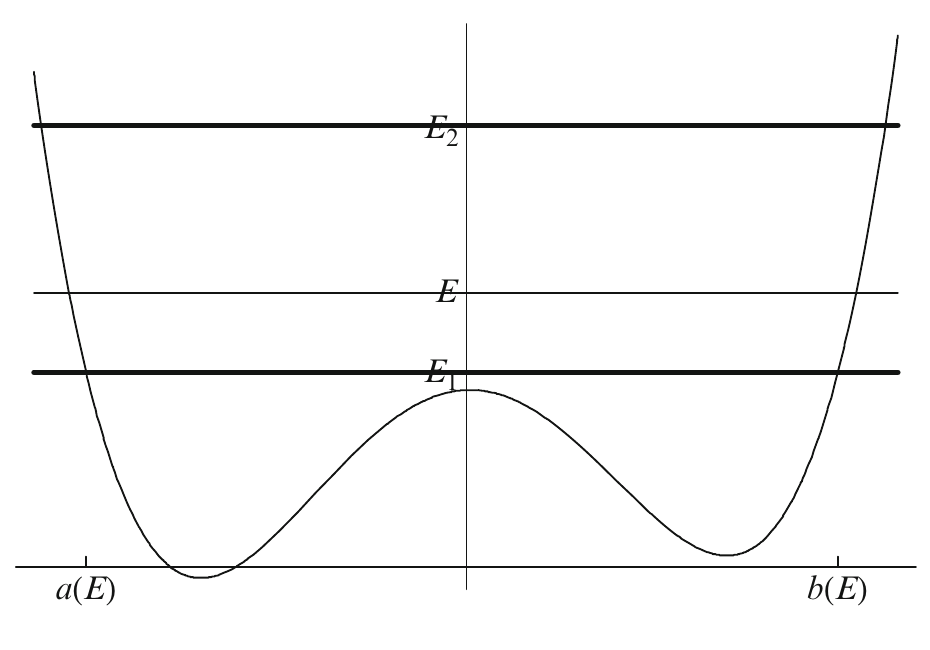
\includegraphics[width=0.76\textwidth]{figures/figure-15-2.png}
\caption{满足假设~\ref{assumption:wkb} 的一个势函数.}
\label{fig:wkb-potential-assumption}
\end{figure}

\subsection{经典允许区间}
\label{subsec:wkb-allowed}

仍取式~\eqref{eq:wkb-ansatz}.由式~\eqref{eq:wkb-first-computation},若希望误差小于 $O(\hbar)$,必须令 $A$ 满足
\[
2A'(x)p(x)=-p'(x)A(x),
\qquad
\frac{A'(x)}{A(x)}=-\frac12\frac{p'(x)}{p(x)}.
\label{eq:wkb-amplitude-ode}
\]
所以(见练习~\ref{ex:wkb-amplitude})
\[
A(x)=C p(x)^{-1/2}.
\label{eq:wkb-amplitude}
\]
此时
\[
\widehat H\psi-E\psi=-\frac{\hbar^2}{2m}\frac{A''(x)}{A(x)}\psi(x).
\label{eq:wkb-local-error}
\]
形式上误差为 $O(\hbar^2)$,但该式只在允许区间局部成立;$p(x)$ 在转向点趋于零,故振幅在转向点发散.

取两个相反指数的线性组合,并把积分基点取为左转向点 $a$.由于 Schrödinger 算子与复共轭对易,可以只考虑实值近似解.

\begin{note}[振荡型 WKB 函数]\label{note:wkb-oscillatory}
在经典允许区间且远离转向点处,实值 Schrödinger 解应近似为
\[
\psi(x)\approx\frac{R}{\sqrt{p(x)}}
\cos\left(\frac1\hbar\int_a^xp(y)\,dy-\delta\right),
\label{eq:wkb-oscillatory}
\]
其中 $R,\delta$ 是实常数,分别称为振幅与相位.
\end{note}

对式~\eqref{eq:wkb-oscillatory} 的平方使用 $\cos^2\theta=(1+\cos2\theta)/2$.小 $\hbar$ 时快速振荡的余弦项因正负抵消而较小,所以概率密度的主导项与 $1/p(x)$ 成正比,即与 $1/v(x)$ 成正比;而 $1/v(x)=dt/dx$,故粒子在某区间内出现的概率近似等于经典粒子在该区间内所用时间占一个周期的比例.

\subsection{经典禁阻区间}
\label{subsec:wkb-forbidden}

令
\[
q(x)=\sqrt{2m(V(x)-E)}.
\]
在经典禁阻区间寻找
\[
\psi(x)=A(x)\exp\left(\pm\frac1\hbar\int q(y)\,dy\right).
\]
同样分析可知,为抵消 $O(\hbar)$ 项,唯一的振幅(相差常数倍)为 $A(x)=Cq(x)^{-1/2}$.在 $(b,+\infty)$ 上,为得到平方可积解取负号并以 $b$ 为积分基点;在 $(-\infty,a)$ 上取正号并反向积分,最终也可写成负指数.

\begin{note}[指数型 WKB 函数]\label{note:wkb-exponential}
若 $\psi_1$ 是趋于 $-\infty$ 时趋于零的定态解,则在 $(-\infty,a)$ 且远离 $a$ 处,
\[
\psi_1(x)\approx\frac{c_1}{\sqrt{q(x)}}
\exp\left(-\frac1\hbar\int_x^a q(y)\,dy\right).
\label{eq:wkb-left-forbidden}
\]
若 $\psi_2$ 是趋于 $+\infty$ 时趋于零的定态解,则在 $(b,+\infty)$ 且远离 $b$ 处,
\[
\psi_2(x)\approx\frac{c_2}{\sqrt{q(x)}}
\exp\left(-\frac1\hbar\int_b^x q(y)\,dy\right).
\label{eq:wkb-right-forbidden}
\]
转向点处的奇异性只是近似方法的产物;真实的光滑势的定态解是光滑的,并且在小 $\hbar$ 下只会在非常靠近转向点时偏离 WKB 近似.
\end{note}

\begin{figure}[htbp]
\centering
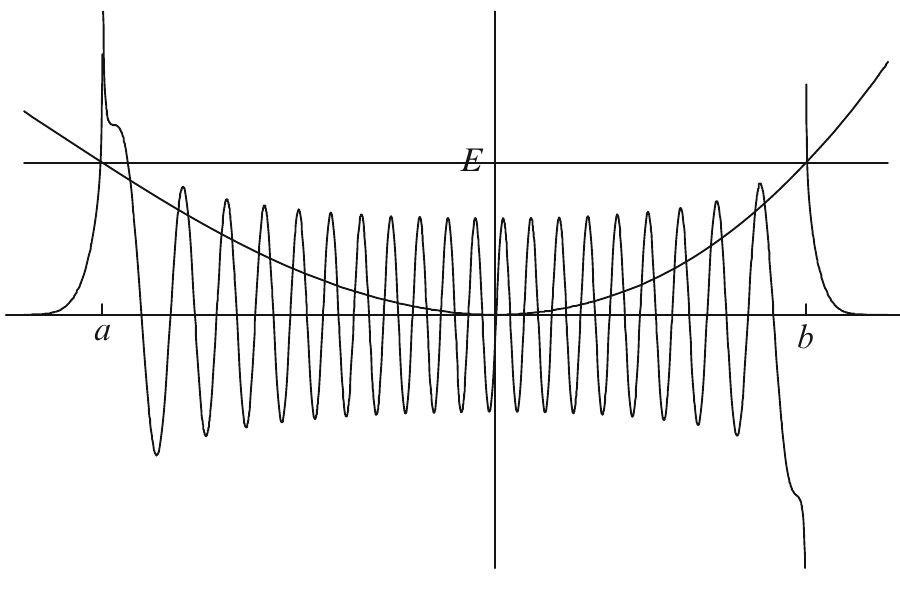
\includegraphics[width=0.76\textwidth]{figures/figure-15-3.png}
\caption{把 WKB 函数一直延拓到转向点.}
\label{fig:wkb-extended-functions}
\end{figure}

\section{Airy 函数与连接公式}
\label{sec:wkb-airy-connection}

若 $\psi_1$ 在 $-\infty$ 处衰减,则它在允许区间的振荡近似中的常数 $R,\delta$ 应当由左转向点附近的连接公式决定.设
\[
F_0=-V'(a)>0,
\qquad V(x)\approx(a-x)F_0.
\]
Schrödinger 方程在 $a$ 附近近似为
\[
-\frac{\hbar^2}{2m}\frac{d^2\psi}{dx^2}+(a-x)F_0\psi=0.
\]
作变量代换
\[
u=\left(\frac{2mF_0}{\hbar^2}\right)^{1/3}(a-x),
\label{eq:wkb-airy-variable}
\]
得到 Airy 方程
\[
\frac{d^2\psi}{du^2}-u\psi(u)=0.
\label{eq:airy-equation}
\]
它有两个线性无关解 $\operatorname{Ai}(u),\operatorname{Bi}(u)$;因为 $\operatorname{Ai}(u)$ 在 $u>0$(即 $x<a$)衰减,我们取
\[
\operatorname{Ai}(u)=\frac1\pi\int_0^\infty\cos\left(\frac{t^3}{3}+ut\right)\,dt.
\label{eq:airy-integral}
\]
积分由快速振荡收敛,严格证明可用练习~\ref{ex:airy-convergence} 的分部积分.对 $u$ 大小的渐近性可由驻相法与反复分部积分得到.

\begin{proposition}[Airy 连接公式]\label{claim:airy-connection}
若 $\psi_1$ 是在 $-\infty$ 附近趋于零的 Schrödinger 方程解,则可归一化使
\begin{align}
\psi_1(x)&\approx\frac1{2\sqrt{q(x)}}\exp\left(-\frac1\hbar\int_x^a q(y)\,dy\right), &&x\to-\infty,\\
\psi_1(x)&\approx\frac{\sqrt\pi}{(2mF_0\hbar)^{1/6}}
\operatorname{Ai}\left(\left(\frac{2mF_0}{\hbar^2}\right)^{1/3}(a-x)\right), &&x\approx a,\\
\psi_1(x)&\approx\frac1{\sqrt{p(x)}}\cos\left(\frac1\hbar\int_a^xp(y)\,dy-\frac\pi4\right), &&a<x<b.
\end{align}
\end{proposition}

类似地,若 $\psi_2$ 在 $+\infty$ 处趋于零,令 $F_1=V'(b)>0$,则
\begin{align}
\psi_2(x)&\approx\frac1{\sqrt{p(x)}}\cos\left(-\frac1\hbar\int_x^bp(y)\,dy+\frac\pi4\right), &&a<x<b,\\
\psi_2(x)&\approx\frac{\sqrt\pi}{(2mF_1\hbar)^{1/6}}
\operatorname{Ai}\left(\left(\frac{2mF_1}{\hbar^2}\right)^{1/3}(x-b)\right), &&x\approx b,\\
\psi_2(x)&\approx\frac1{2\sqrt{q(x)}}\exp\left(-\frac1\hbar\int_b^xq(y)\,dy\right), &&x\to+\infty.
\end{align}

\begin{figure}[htbp]
\centering
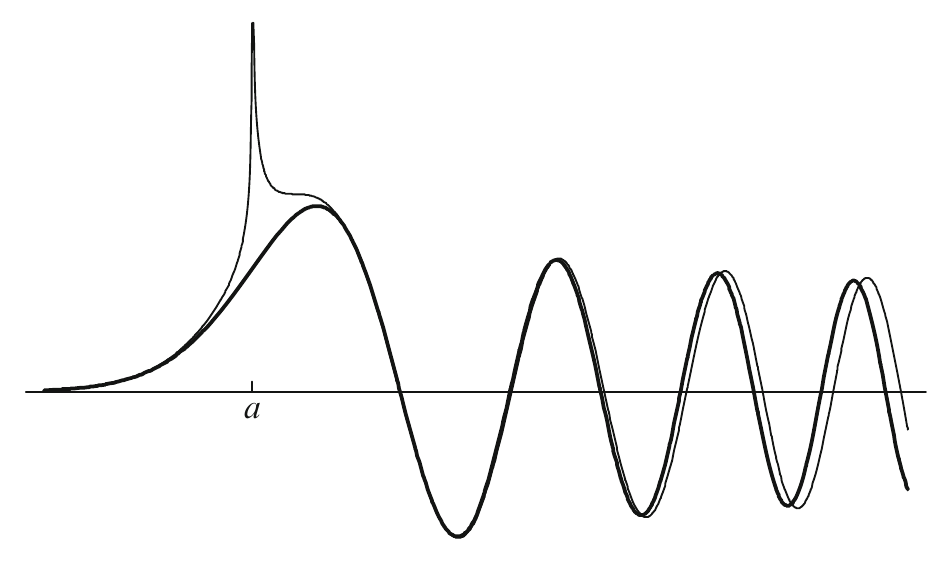
\includegraphics[width=0.76\textwidth]{figures/figure-15-4.png}
\caption{转向点 $x=a$ 附近缩放后的 Airy 函数(粗曲线)与 WKB 函数.}
\label{fig:wkb-airy-wkb-comparison}
\end{figure}

\begin{figure}[htbp]
\centering
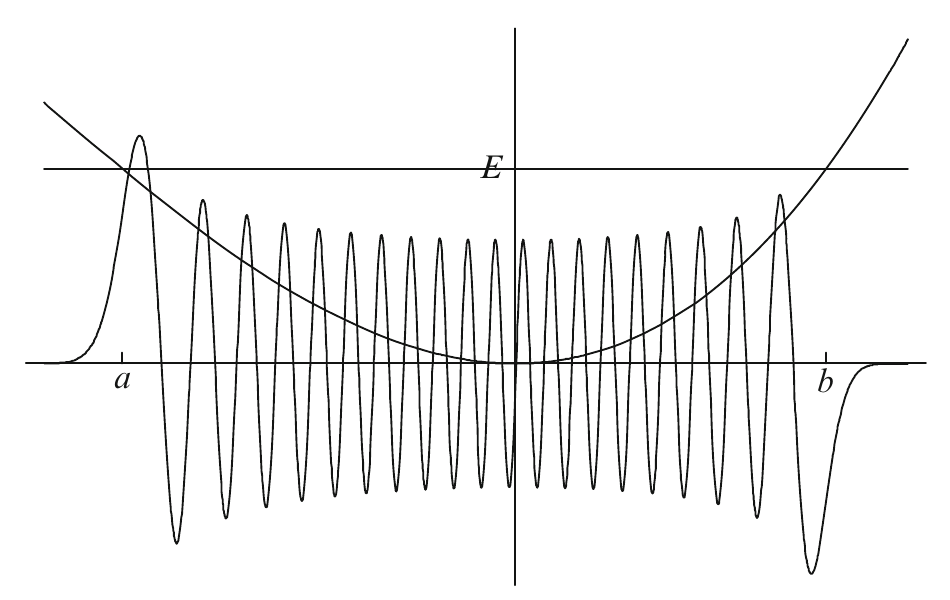
\includegraphics[width=0.76\textwidth]{figures/figure-15-5.png}
\caption{$n=39$ 时的近似波函数.}
\label{fig:wkb-approximate-wavefunction}
\end{figure}

\begin{figure}[htbp]
\centering
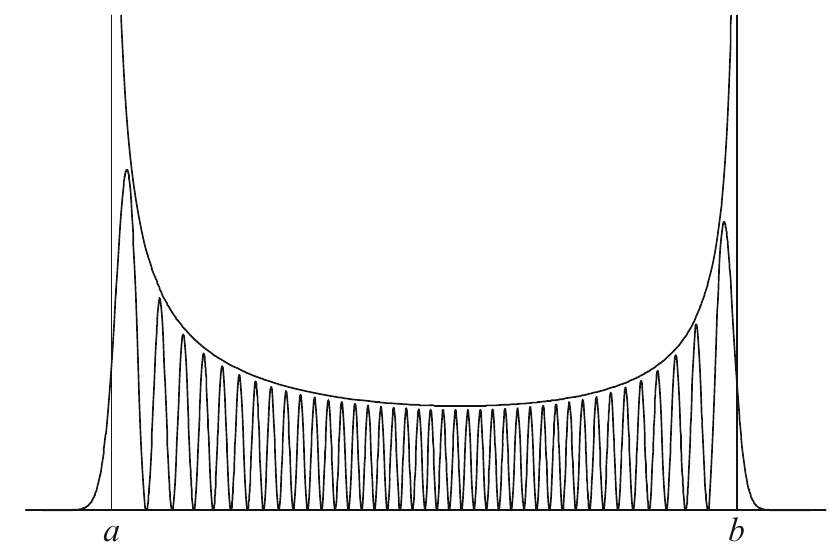
\includegraphics[width=0.76\textwidth]{figures/figure-15-6.png}
\caption{近似波函数的概率分布与函数 $1/p(x)$ 的比较.}
\label{fig:wkb-probability-distribution}
\end{figure}

Airy 函数的两条渐近公式为
\[
\operatorname{Ai}(u)\approx\frac1{2\sqrt\pi}u^{-1/4}e^{-2u^{3/2}/3},
\qquad u\to+\infty,
\label{eq:airy-positive-asymptotic}
\]
以及
\[
\operatorname{Ai}(u)\approx\frac1{\sqrt\pi(-u)^{1/4}}
\cos\left(\frac23(-u)^{3/2}-\frac\pi4\right),
\qquad u\to-\infty.
\label{eq:airy-negative-asymptotic}
\]
在左转向点附近的线性近似给出
\[
p(x)\approx\sqrt{2mF_0}\sqrt{x-a},
\qquad
\frac1\hbar\int_a^xp(y)\,dy\approx\frac23(-u)^{3/2}.
\]
代入式~\eqref{eq:airy-negative-asymptotic} 即得到左连接公式;式~\eqref{eq:airy-positive-asymptotic} 给出禁阻区间的指数型公式.右转向点同理.

\begin{proposition}[WKB 能量匹配条件]\label{prop:wkb-matching-condition}
左右两侧得到的允许区间近似解当且仅当存在非负整数 $n$,使
\[
\frac1\hbar\int_a^bp(x)\,dx=\left(n+\frac12\right)\pi.
\label{eq:wkb-matching}
\]
该条件等价于定义~\ref{condition:maslov-bohr-sommerfeld} 中的 Maslov 修正 Bohr--Sommerfeld 条件.若 $n$ 为偶数,左右近似解相等;若 $n$ 为奇数,它们互为相反数.
\end{proposition}

\begin{proof}
令
\[
\phi=\frac1\hbar\int_a^bp(y)\,dy-\frac\pi2.
\]
左侧相位与右侧相位相差 $\phi$.当 $\phi$ 为 $\pi$ 的偶数倍或奇数倍时,两个余弦分别相等或互为相反数;其他情形下,一个余弦函数不可能是另一个余弦函数的常数倍(见练习~\ref{ex:wkb-phase}).故式~\eqref{eq:wkb-matching} 是必要且充分的.
\end{proof}

\section{严格误差估计}
\label{sec:wkb-rigorous-error}

前面的各节给出了许多教材中常见的 WKB 近似处理.这样的处理说明:满足修正 Bohr--Sommerfeld 条件(条件~\ref{condition:maslov-bohr-sommerfeld})的能量应该是 Hamilton 算子 $\widehat H$ 的近似特征值,但还没有说明“近似”究竟具有什么严格含义.本节证明如下的估计.

\begin{theorem}[WKB 近似的严格误差估计]\label{thm:wkb-rigorous-error}
对满足假设~\ref{assumption:wkb} 的任意势函数 $V$ 与能量范围 $[E_1,E_2]$,存在常数 $C$,使得:对 $[E_1,E_2]$ 中满足条件~\ref{condition:maslov-bohr-sommerfeld} 的任意能量 $E$,都存在非零函数 $\psi\in\operatorname{Dom}(\widehat H)$,满足
\[
\|\widehat H\psi-E\psi\|<C\hbar^{9/8}\|\psi\|.
\label{eq:wkb-rigorous-residual}
\]
\end{theorem}

如第~\ref{sec:wkb-classical-semiclassical} 节已经指出,若存在满足
$\|\widehat H\psi-E\psi\|<\varepsilon\|\psi\|$ 的函数,则 $\widehat H$ 的谱中存在某个 $\widetilde E$,使 $|E-\widetilde E|<\varepsilon$(见第 10 章练习 4).由于在假设~\ref{assumption:wkb} 下 $\widehat H$ 的谱纯离散,我们得到:对于每个满足条件~\ref{condition:maslov-bohr-sommerfeld} 的 $E\in[E_1,E_2]$,$\widehat H$ 都有一个真正的特征值 $\widetilde E$,满足
\[
|E-\widetilde E|<C\hbar^{9/8}.
\label{eq:wkb-eigenvalue-error}
\]

如果 $E$ 满足条件~\ref{condition:maslov-bohr-sommerfeld},实际上可以证明式~\eqref{eq:wkb-eigenvalue-error} 右侧的 $\hbar^{9/8}$ 可替换为 $\hbar^2$.不过,用本章的方法不可能得到这样的最优估计:本定理证明中构造的近似特征向量并不满足 $\|\widehat H\psi-E\psi\|<C\hbar^2\|\psi\|$.另一方面,可以用其他方法(例如参考文献~[31] 中的方法)构造出误差为 $O(\hbar^2)$ 的近似特征向量.尽管如此,式~\eqref{eq:wkb-eigenvalue-error} 中的误差相对于能级的典型间距仍然很小,因为后者的数量级为 $\hbar$.

回忆假设~\ref{assumption:wkb}:势函数光滑并且在两端趋于 $+\infty$ 的 Schrödinger 算子在 $C_c^\infty(\mathbb R)$ 上本质自伴.本定理中的 $\widehat H$ 更准确地说,是定义在 $C_c^\infty(\mathbb R)$ 上的 Schrödinger 算子的唯一自伴延拓.

\subsection{准备工作}
\label{subsec:wkb-rigorous-preliminaries}

近似特征函数 $\psi$ 的构造基本按照命题~\ref{claim:airy-connection} 中概述的 WKB 近似进行:在转向点附近使用缩放后的 Airy 函数,在经典允许区间和禁阻区间使用标准 WKB 函数.不过,这种做法存在一个困难:缩放后的 Airy 函数在不同区域的边界处并不与 WKB 函数完全相同,而只是近似相同.于是,如果在形如 $(-\infty,a-\varepsilon)$ 的区间上用 WKB 公式定义 $\psi$,在 $(a-\varepsilon,a+\varepsilon)$ 上用缩放后的 Airy 函数定义 $\psi$,那么 $\psi$ 在 $a-\varepsilon$ 处可能不连续.即使在某个区间上乘以常数消除了 $\psi$ 本身的不连续,其导数通常仍会不连续.但如果 $\psi'$ 不连续,$\psi$ 就不属于 $\widehat H$ 的定义域,式~\eqref{eq:wkb-rigorous-residual} 的左端也就没有意义(可与第 5 章相应讨论比较).

要求 $\psi'$ 连续并不只是技术细节.如果不关心导数的连续性,就可以无论能量是否满足修正 Bohr--Sommerfeld 条件,都通过分别乘以常数把缩放后的 Airy 函数与 WKB 函数接起来.那样就会错误地声称 $[E_1,E_2]$ 中的任意 $E$ 都距 $\widehat H$ 的某个特征值至多 $C\hbar^{9/8}$;对谐振子而言这显然是错误的.

为克服上述困难,必须加入过渡区,在其中用光滑方式从一个函数过渡到另一个函数;这就是小节~\ref{subsec:wkb-transition-regions} 中的“拼接”构造.具体地说,在命题~\ref{claim:airy-connection} 所列的区间内使用相应公式,并在 $n$ 为奇数时把相应的允许区间函数及右侧匹配函数乘以 $-1$.在 $(a-\varepsilon,a+\varepsilon)$ 和 $(b-\varepsilon,b+\varepsilon)$ 上分别使用缩放后的 Airy 函数,再加入四个长度为 $\delta$ 的过渡区;$\varepsilon,\delta$ 随 $\hbar$ 的具体选择将在下面给出.图~\ref{fig:wkb-approximate-eigenfunction} 示意了转向点 $x=a$ 附近的过渡区.

\begin{figure}[htbp]
\centering
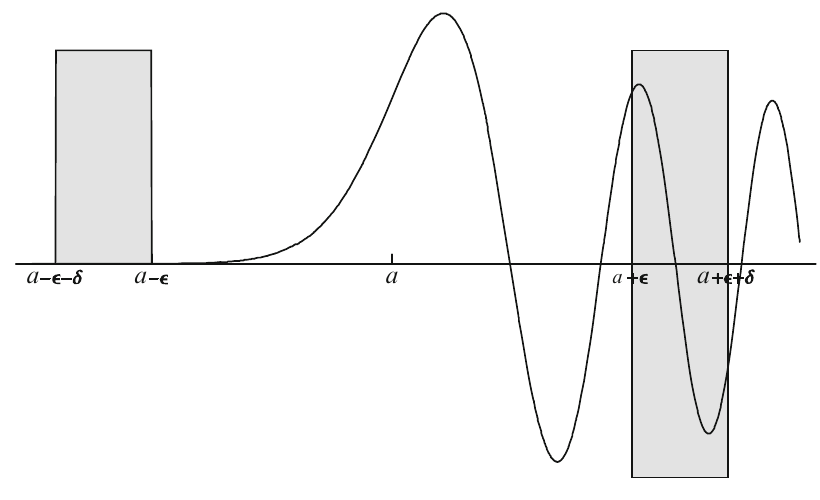
\includegraphics[width=0.78\textwidth]{figures/figure-15-7.png}
\caption{带有阴影过渡区的近似特征函数 $\psi$.}
\label{fig:wkb-approximate-eigenfunction}
\end{figure}

设 $\widehat H_0$ 是势函数为 $V$、定义域为 $C_c^\infty(\mathbb R)$ 的 Schrödinger 算子.由前面的讨论,$\widehat H_0$ 本质自伴;令 $\widehat H$(与伴随算子 $\widehat H_0^*$ 一致)表示它的唯一自伴延拓.$\widehat H_0^*$ 的定义域由所有满足以下条件的 $\psi\in L^2(\mathbb R)$ 组成:以分布意义计算的 Schrödinger 算子作用于 $\psi$ 后仍属于 $L^2(\mathbb R)$.特别地,如果 $\psi$ 光滑,则 $\psi\in\operatorname{Dom}(\widehat H)=\operatorname{Dom}(\widehat H_0^*)$ 当且仅当 $\psi\in L^2(\mathbb R)$ 且
\[
-\frac{\hbar^2}{2m}\psi''+V\psi\in L^2(\mathbb R).
\label{eq:wkb-domain-criterion}
\]

由于使用了拼接,构造出的近似特征函数 $\psi$ 在整个 $\mathbb R$ 上实际上是无穷可微的.又因为 $V(x)$ 在两端趋于 $+\infty$,指数型 WKB 函数在无穷远处快速衰减,所以 $\psi\in L^2(\mathbb R)$.在 $x$ 接近两端无穷远处,前面的计算(式~\eqref{eq:wkb-local-error})适用;取 $A(x)=Cq(x)^{-1/2}$,直接计算得到
\[
-\frac{\hbar^2}{2m}\psi''(x)+V(x)\psi(x)
=-\frac{\hbar^2}{2m}\left[
\frac5{16}\left(\frac{V'(x)}{V(x)-E}\right)^2
-\frac14\frac{V''(x)}{V(x)-E}
\right]\psi(x).
\label{eq:wkb-domain-error}
\]
由于假设 $V'/V$ 与 $V''/V$ 在无穷远处有界,且 $V(x)\to+\infty$,上式说明在无穷远处 Schrödinger 算子作用于 $\psi$ 的结果被 $\psi$ 的常数倍控制,因而属于平方可积函数.这证明了 $\psi\in\operatorname{Dom}(\widehat H)$.

在小节~\ref{subsec:wkb-turning-point-regions} 中,我们将取转向点附近区间的宽度 $2\varepsilon$ 为 $O(\hbar^{1/2})$.尽管 Airy 函数在非常靠近转向点处有 $O(\hbar^{-1/6})$ 的发散,近似波函数的 $L^2$ 范数在 $\hbar\to0$ 时仍为 $O(1)$(有正的下界且有有限上界).这不难验证(见练习~\ref{ex:wkb-norm});即便范数发散,也只会使证明 $\|\widehat H\psi-E\psi\|$ 相对于 $\|\psi\|$ 很小变得更容易.

为了证明定理~\ref{thm:wkb-rigorous-error},必须分别估计四类区域对 $\|\widehat H\psi-E\psi\|$ 的贡献:经典允许区间、经典禁阻区间、转向点附近的区域以及过渡区.下面各小节将完成这些估计,其中过渡区的分析最为复杂.特别重要的是,在过渡区内缩放后的 Airy 函数的导数必须几乎与 WKB 函数的导数匹配,这正是引理~\ref{lem:wkb-transition-mismatch} 的第二部分.

\subsection{转向点附近的区域}
\label{subsec:wkb-turning-point-regions}

在每个转向点附近的区间内使用缩放后的 Airy 函数(在 $x=a$ 附近使用式~\eqref{eq:wkb-airy-variable} 所对应的函数,在 $x=b$ 附近则根据 $n$ 的奇偶性使用相应函数或其相反数).下面验证,取这些区间的长度为 $O(\hbar^{1/2})$ 会得到足够好的估计.

若 $\psi$ 是其中一个缩放后的 Airy 函数,则它满足一个把势函数 $V$ 换成转向点附近线性近似 $\widetilde V$ 的 Schrödinger 方程.因此
\[
\widehat H\psi-E\psi=(V(x)-\widetilde V(x))\psi.
\label{eq:wkb-turning-residual}
\]
势函数 $V$ 与线性近似 $\widetilde V$ 的差至多按距转向点的距离的平方增长.另一方面,Airy 函数的渐近式给出 $|\operatorname{Ai}(u)|\leq Cu^{-1/4}$(对小 $u$ 来说这是很差的估计,但仍然成立).式~\eqref{eq:wkb-airy-variable} 中的 $u$ 的数量级为 $\hbar^{-2/3}$ 乘以距转向点的距离;式中的缩放因子还有 $\hbar^{-1/6}$,而距转向点至多为 $O(\hbar^{1/2})$.因此,在转向点附近区间上
\[
|\widehat H\psi-E\psi|
\leq C(\hbar^{1/2})^2\hbar^{-1/6}
\bigl(\hbar^{-2/3}\hbar^{1/2}\bigr)^{-1/4}
=C\hbar^{7/8}.
\]
若函数 $f$ 在长度为 $L$ 的区间上满足 $|f|\leq D$,则其在该区间上的 $L^2$ 范数至多为 $D\sqrt L$.所以转向点附近区域的贡献为
\[
\|\widehat H\psi-E\psi\|=O(\hbar^{7/8}\hbar^{1/4})=O(\hbar^{9/8}).
\label{eq:wkb-turning-error}
\]

\subsection{经典允许区间与经典禁阻区间}
\label{subsec:wkb-allowed-forbidden-error}

由式~\eqref{eq:wkb-domain-error}(它由式~\eqref{eq:wkb-local-error} 得到)给出的表达式,在经典允许区间和禁阻区间都适用.先考虑经典允许区间.虽然式~\eqref{eq:wkb-domain-error} 形式上是 $O(\hbar^2)$,但我们是在端点随 $\hbar\to0$ 逐渐靠近转向点的区间上使用它;而且式中的表达式在转向点处发散,所以这一段对 $\|\widehat H\psi-E\psi\|$ 的贡献会大于 $\hbar^2$ 的数量级.

转向点附近区间的宽度 $2\varepsilon$ 取为 $O(\hbar^{1/2})$,并且下面还会取过渡区宽度 $\delta=O(\hbar^{1/2})$.因此,在经典允许区间中使用振荡型 WKB 函数的区间可写成 $(a+\gamma,b-\gamma)$,其中 $\gamma=\varepsilon+\delta=O(\hbar^{1/2})$.

允许区间中的 $\psi$ 含有 $p(x)^{-1/2}$ 因子和有界的余弦因子.由于 $V'(a)\neq0$,当 $x\to a$ 时,$V(x)-E$ 的行为与 $x-a$ 成正比,从而 $p(x)^{-1/2}$ 与 $(x-a)^{-1/4}$ 成正比;在另一个转向点附近也有类似行为.另一方面,式~\eqref{eq:wkb-domain-error} 中问题最大的项含有 $(V(x)-E)^{-2}$,再考虑 $\psi$ 自身的 $p(x)^{-1/2}$ 发散,该项在 $a$ 附近的行为为 $(x-a)^{-9/4}$.于是,在允许区间左半段可估计为
\[
\begin{aligned}
\|\widehat H\psi-E\psi\|&\leq C\hbar^2
\left(\int_{a+\gamma}^{(a+b)/2}(x-a)^{-9/2}\,dx\right)^{1/2}\\
&=C'\hbar^2\left(\gamma^{-7/2}-\left(\frac{a+b}{2}-a\right)^{-7/2}\right)^{1/2}.
\end{aligned}
\]
由于 $\gamma=O(\hbar^{1/2})$,该贡献的主导项为 $\hbar^2\hbar^{-7/8}=\hbar^{9/8}$;允许区间的另一半同理.

在第一个经典禁阻区间中也使用式~\eqref{eq:wkb-domain-error}.由假设~\ref{assumption:wkb},$V'/V$ 与 $V''/V$ 在无穷远处有界;因此 $V'/(V-E)$ 与 $V''/(V-E)$ 在无穷远处也有界,并且在 $(-\infty,a-1)$ 上有界,因为 $V-E$ 在该区间严格为正且在 $x\to-\infty$ 时趋于 $+\infty$.所以该区间上 $\|\widehat H\psi-E\psi\|$ 至多为常数乘以 $\hbar^2\|\psi\|$.在 $(a-1,a-\gamma)$ 上的估计与允许区间相似,但此处还有 WKB 函数的指数衰减因子,因此经典禁阻区间 $(-\infty,a-\gamma)$ 的贡献肯定不超过 $O(\hbar^{9/8})$;右侧禁阻区间同理.

\subsection{过渡区}
\label{subsec:wkb-transition-regions}

给定两个光滑函数 $\psi_1,\psi_2$ 以及形如 $[\alpha,\alpha+\delta]$ 的区间,定义它们的“拼接” $\psi_1;\psi_2$:当 $x<\alpha$ 时等于 $\psi_1(x)$,当 $x>\alpha+\delta$ 时等于 $\psi_2(x)$,并且在整个实轴上光滑.取 $[0,1]$ 上的光滑函数 $\chi$,使其在 $0$ 的某邻域恒为 $0$、在 $1$ 的某邻域恒为 $1$.定义
\[
(\psi_1;\psi_2)(x)=\psi_1(x)+(\psi_2(x)-\psi_1(x))\chi\left(\frac{x-\alpha}{\delta}\right).
\label{eq:wkb-join}
\]

图~\ref{fig:wkb-join} 给出了示意图.直接计算得到
\[
\begin{aligned}
(\widehat H-EI)(\psi_1;\psi_2)
={}&(\widehat H\psi_1-E\psi_1);(\widehat H\psi_2-E\psi_2)\\
&-\frac{\hbar^2}{m\delta}(\psi_2'(x)-\psi_1'(x))\chi'\left(\frac{x-\alpha}{\delta}\right)\\
&-\frac{\hbar^2}{2m\delta^2}(\psi_2(x)-\psi_1(x))\chi''\left(\frac{x-\alpha}{\delta}\right).
\end{aligned}
\label{eq:wkb-join-error}
\]

\begin{figure}[htbp]
\centering
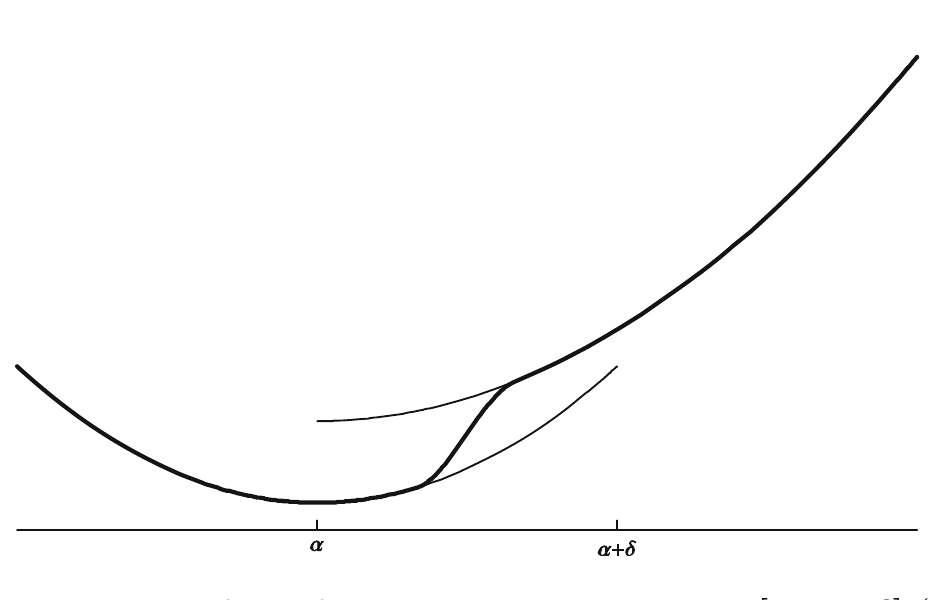
\includegraphics[width=0.78\textwidth]{figures/figure-15-8.png}
\caption{在区间 $[\alpha,\alpha+\delta]$ 上拼接两个函数;粗曲线表示拼接函数.}
\label{fig:wkb-join}
\end{figure}

我们在五个不同区域使用五种不同公式:两个经典禁阻区间、一个经典允许区间以及两个转向点附近的区域.由于相邻区间中的函数并不完全匹配,必须使用四次拼接,才能得到属于 $\widehat H$ 定义域的函数.拼接区间的宽度 $\delta$ 取为与转向点附近区间相同的数量级,即 $O(\hbar^{1/2})$.

最关键的情况是从转向点附近区域过渡到经典允许区间.以左转向点为例,令 $\psi_1$ 为式~\eqref{eq:wkb-airy-variable} 对应的缩放 Airy 函数,令 $\psi_2$ 为振荡型 WKB 函数.二者的不匹配有两个来源:第一,Airy 函数与其主导渐近式之间存在差异;第二,式~\eqref{eq:airy-negative-asymptotic} 与连接公式中所用的近似,忽略了势函数 $V$ 与其在 $x=a$ 处的线性近似 $\widetilde V$ 之间的差异.估计 $\psi_1-\psi_2$ 及其导数时,必须同时考虑这两项.

\begin{lemma}[过渡区中的 Airy--WKB 匹配]\label{lem:wkb-transition-mismatch}
令 $\psi_1$ 是左转向点处的缩放 Airy 函数,令 $\widetilde\psi_1$ 是把其中的 Airy 函数替换为式~\eqref{eq:airy-negative-asymptotic} 右端所得的函数,令 $\psi_2$ 是振荡型 WKB 函数.当 $x-a$ 为 $O(\hbar^{1/2})$ 时,有
\[
|\psi_1(x)-\widetilde\psi_1(x)|=O(\hbar^{1/8}),
\qquad
|\widetilde\psi_1(x)-\psi_2(x)|=O(\hbar^{1/8}),
\label{eq:wkb-function-mismatch}
\]
且
\[
|\psi_1'(x)-\widetilde\psi_1'(x)|=O(\hbar^{-5/8}),
\qquad
|\widetilde\psi_1'(x)-\psi_2'(x)|=O(\hbar^{-5/8}).
\label{eq:wkb-derivative-mismatch}
\]
\end{lemma}

先说明这个引理的估计足以控制转向点附近区域 $(a+\varepsilon,a+\varepsilon+\delta)$ 对误差的贡献,其中 $\varepsilon,\delta=O(\hbar^{1/2})$.拼接误差式~\eqref{eq:wkb-join-error} 的第一行的 $L^2$ 范数至多为 $O(\hbar^{9/8})$,理由与小节~\ref{subsec:wkb-allowed-forbidden-error} 中相同.若函数在长度为 $L$ 的区间上绝对值不超过 $C$,则其 $L^2$ 范数至多为 $C\sqrt L$.因此,第二行的 $L^2$ 范数为
\[
O\left(\delta^{-1}\hbar^2\hbar^{-5/8}\delta^{1/2}\right)
=O(\hbar^{9/8}),
\]
而第三行的贡献为
\[
O\left(\delta^{-2}\hbar^2\hbar^{1/8}\delta^{1/2}\right)
=O(\hbar^{11/8}).
\]
所以该过渡区的总贡献至多为 $O(\hbar^{9/8})$.从经典允许区间过渡到右转向点附近区域的分析完全相同.转向点附近区域与经典禁阻区间之间的过渡则容易得多,因为参与拼接的所有函数在过渡区内都很小.例如,当 $a-x=O(\hbar^{1/2})$ 时,Airy 变量 $u$ 为 $O(\hbar^{-1/6})$,因而 $u^{3/2}=O(\hbar^{-1/4})$;$u>0$ 时 Airy 函数渐近式中的指数因子形如 $\exp(-C\hbar^{-1/4})$,对小 $\hbar$ 而言比任意幂次的 $\hbar$ 都小.因此这些过渡区的贡献小于任意给定的 $\hbar$ 幂次,当然不会超过 $O(\hbar^{9/8})$.

\begin{proof}
我们只证明引理中关于导数的估计;关于函数本身的估计类似而且更容易,留给练习~\ref{ex:wkb-mismatch-functions}.

先考虑 $\psi_1'-\widetilde\psi_1'$.直接计算得到
\[
\psi_1'(x)-\widetilde\psi_1'(x)
=-\sqrt\pi(2mF_0)^{1/6}\hbar^{-5/6}
\left(\operatorname{Ai}'(u)-\widetilde{\operatorname{Ai}}'(u)\right),
\label{eq:wkb-airy-derivative-difference}
\]
其中 $u$ 如式~\eqref{eq:wkb-airy-variable},$\widetilde{\operatorname{Ai}}$ 表示式~\eqref{eq:airy-negative-asymptotic} 右端的函数.

当 $u\to-\infty$ 时,$\operatorname{Ai}(u)$ 有渐近展开
\[
\widetilde{\operatorname{Ai}}(u)=\operatorname{Ai}(u)\bigl(1+O((-u)^{-3/2})\bigr),
\]
而 $\operatorname{Ai}'(u)$ 的展开可由对上式关于 $u$ 形式求导得到.因此
\[
\operatorname{Ai}'(u)-\widetilde{\operatorname{Ai}}'(u)
=\widetilde{\operatorname{Ai}}'(u)O((-u)^{-3/2})
+\widetilde{\operatorname{Ai}}(u)O((-u)^{-5/2}).
\label{eq:wkb-airy-asymptotic-error}
\]
从显式公式看,$\widetilde{\operatorname{Ai}}(u)$ 的数量级为 $(-u)^{-1/4}$,而 $\widetilde{\operatorname{Ai}}'(u)$ 含有一个数量级为 $(-u)^{1/4}$ 的主导项.所以式~\eqref{eq:wkb-airy-asymptotic-error} 右端衰减较慢的项为 $O((-u)^{-5/4})$.在过渡区,$u=O(\hbar^{-2/3}\hbar^{1/2})=O(\hbar^{-1/6})$,故式~\eqref{eq:wkb-airy-derivative-difference} 的数量级为
\[
\hbar^{-5/6}\hbar^{5/24}=\hbar^{-5/8},
\]
得到所需估计.

再考虑 $\widetilde\psi_1'-\psi_2'$.直接计算可知,$\widetilde\psi_1'$ 和 $\psi_2'$ 都由两项组成:对余弦因子求导得到的“主导项”,以及对余弦前系数求导得到的“次主导项”.在 $\widetilde\psi_1'$ 中,主导项可化为
\[
-\frac1\hbar\bigl((2mF_0)(x-a)\bigr)^{1/4}
\sin\left(\frac23(-u)^{3/2}-\frac\pi4\right).
\label{eq:wkb-airy-dominant-derivative}
\]
练习~\ref{ex:wkb-phase-expansion} 将证明,当 $x-a=O(\hbar^{1/2})$ 时
\[
\bigl((2mF_0)(x-a)\bigr)^{1/4}=\sqrt{p(x)}\bigl(1+O(\hbar^{1/2})\bigr),
\label{eq:wkb-amplitude-comparison}
\]
以及
\[
\frac23(-u)^{3/2}=\frac1\hbar\int_a^xp(y)\,dy+O(\hbar^{1/4}).
\label{eq:wkb-phase-comparison}
\]
由于 $\sin\theta$ 的导数有界,正弦函数自变量改变 $O(\hbar^{1/4})$ 时,函数值也只改变 $O(\hbar^{1/4})$.把式~\eqref{eq:wkb-amplitude-comparison} 与式~\eqref{eq:wkb-phase-comparison} 代入式~\eqref{eq:wkb-airy-dominant-derivative},两主导项的差为
\[
\frac1\hbar\sqrt{p(x)}O(\hbar^{1/4})+\text{更低阶项}.
\]
由于 $\sqrt{p(x)}$ 的数量级为 $(x-a)^{1/4}$,在过渡区为 $O(\hbar^{1/8})$,故误差为 $O(\hbar^{-5/8})$.最后,$\widetilde\psi_1'$ 和 $\psi_2'$ 中的次主导项分别容易看出也都是 $O(\hbar^{-5/8})$,所以即使不利用它们之间的抵消,也不改变估计的数量级.
\end{proof}

\subsection{主定理的证明}
\label{subsec:wkb-main-theorem-proof}

上面已经分别估计了经典允许区间和禁阻区间、转向点附近区域以及过渡区对 $\|\widehat H\psi-E\psi\|$ 的贡献;每一项都至多为 $O(\hbar^{9/8}\|\psi\|)$.因此只需验证这些估计中的常数在能量范围 $E_1\leq E\leq E_2$ 上一致有界.

这一点是直接的.例如在左转向点 $a$ 附近,由 Taylor 余项公式,$V(x)$ 与线性近似 $\widetilde V(x)$ 的差满足
\[
|V(x)-\widetilde V(x)|\leq\frac12 C|x-a|^2,
\]
其中 $C$ 是从 $a$ 到 $x$ 的区间上 $|V''|$ 的最大值.当 $E$ 在 $[E_1,E_2]$ 中变化时,需要考察 $V''$ 的点集是有界的,故 $C$ 可以取为与 $E$ 无关的常数.

类似地,在经典允许区间中,$1/(V(x)-E)^2$ 在 $x=a(E)$ 附近的发散可以用 $a(E)$ 与 $x$ 之间区间上 $|V'|$ 的最小值控制.由假设,在 $E_1\leq E\leq E_2$ 时所有转向点 $a(E),b(E)$ 处都有 $|V'|>0$;再由连续性,在这些转向点集合的某个邻域内仍有统一的正下界.因此,可取足够小的 $\alpha>0$,使得相关最小值由区间 $[a(E_2)+\alpha,a(E_1)+\alpha]$ 上 $|V'|$ 的最小值控制.其余细节留给读者.

\section{其他方法}
\label{sec:wkb-other-approaches}

WKB 近似的主要复杂性来自转向点附近的奇异行为.然而,转向点之所以造成困难,是因为我们在位置表象中工作.毕竟,转向点只是经典轨道上粒子位置达到最大值或最小值的点;如果改在动量表象中工作,那么动量达到最大值或最小值的点反而会成为问题点.A.~Voros 提议在 Segal--Bargmann 表象(见第~\ref{sec:segal-bargmann} 节)中工作.在 Voros 的分析中不存在转向点,因此分析大为简单.

Voros 方法的问题在于,它只在经典能量曲线上给出波函数的近似.即使在简单情形下,Voros 的表达式也不能全平面延拓为全纯函数,而是在经典能量曲线内部出现分支行为.因此,Voros 公式并不定义量子 Hilbert 空间中的元素(该空间由整函数组成),更不必说定义 Hamilton 算子定义域中的元素了.

尽管如此,仍然可以用相干态的叠加构造近似特征函数,所用公式与 Voros 的公式相似.这种方法避免了处理转向点,同时仍可得到严格的特征值估计,并且使用与条件~\ref{condition:maslov-bohr-sommerfeld} 相同的修正 Bohr--Sommerfeld 条件.见参考文献~[31,23,7];更一般的结果见参考文献~[26].

\section{习题}
\label{sec:wkb-exercises}

\begin{exercise}[复指数的余弦表示]\label{ex:wkb-cosine-combination}
证明:对任意复数 $c_1$,都存在实数 $R,\delta$,使
\[
c_1e^{i\theta}+\overline{c_1}e^{-i\theta}=R\cos(\theta-\delta).
\]
\end{exercise}

\begin{exercise}[谐振子的修正 Bohr--Sommerfeld 条件]\label{ex:wkb-harmonic-bohr-sommerfeld}
设
\[
H(x,p)=\frac{p^2}{2m}+\frac{m\omega^2x^2}{2}
\]
是质量为 $m$、经典频率为 $\omega$ 的谐振子 Hamilton 函数.证明:正数 $E$ 满足修正 Bohr--Sommerfeld 条件~\ref{condition:maslov-bohr-sommerfeld},当且仅当
\[
E=\left(n+\frac12\right)\hbar\omega,
\qquad n\in\mathbb Z_{\geq0}.
\]
\begin{note}[说明]\label{note:wkb-harmonic-exact}
结合第 11 章的结果,这个计算说明,在这个特殊情形中,修正 Bohr--Sommerfeld 条件给出了量子 Hamilton 算子的精确特征值.
\end{note}
\end{exercise}

\begin{exercise}[WKB 振幅方程]\label{ex:wkb-amplitude}
设 $A$ 与 $p$ 是满足式~\eqref{eq:wkb-amplitude-ode} 的两个非零光滑函数.证明存在常数 $C$,使 $A(x)=C p(x)^{-1/2}$.提示:考虑这些函数的对数.
\end{exercise}

\begin{exercise}[余弦相位的唯一性]\label{ex:wkb-phase}
证明:把 $\cos(\theta-\delta)$ 看作 $\theta$ 的函数,它与 $\cos(\theta-\delta')$ 相差一个常数倍,当且仅当 $\delta-\delta'$ 是 $\pi$ 的整数倍.
\end{exercise}

\begin{exercise}[解析延拓的振幅误差]\label{ex:wkb-analytic-continuation}
若 $\psi$ 是 $\widehat H$ 的特征向量,并且在 $-\infty$ 附近由式~\eqref{eq:wkb-left-forbidden} 近似,可以设想在复平面中绕过转向点作解析延拓,从而猜测经典允许区间中的近似表达式.即使 $V$ 是解析的,在上半平面和下半平面作解析延拓也显然不会给出相同答案;但可以把二者的平均作为一个完全非严格的猜测.证明:上述方法给出连接公式中的正确相位 $\delta$,但振幅 $R$ 差一个因子 $2$.
\end{exercise}

\begin{exercise}[Airy 积分的收敛性]\label{ex:airy-convergence}
用分部积分证明极限
\[
\lim_{A\to+\infty}\int_0^A\cos\left(\frac{t^3}{3}+ut\right)\,dt
\]
存在.提示:乘上并除以 $t^2+u$;当 $u<0$ 时避开 $t^2+u=0$ 的点.
\end{exercise}

\begin{exercise}[验证 Airy 方程]\label{ex:airy-equation-verification}
设 Airy 函数由式~\eqref{eq:airy-integral} 给出.假定可以在积分号下微分,验证它满足微分方程
\[
\operatorname{Ai}''(u)-u\operatorname{Ai}(u)=0.
\]
提示:在积分号下微分后,寻找一个可以显式积分的项.更严格的证明可以像练习~\ref{ex:airy-convergence} 那样先分部积分再在积分号下微分,但过程略显繁琐.
\end{exercise}

\begin{exercise}[Airy 函数的快速衰减]\label{ex:airy-rapid-decay}
在式~\eqref{eq:airy-integral} 中反复分部积分,证明当 $u\to+\infty$ 时,$\operatorname{Ai}(u)$ 比 $u$ 的任意负幂都衰减得更快.关键是证明每一步分部积分产生的边界项都为零;积分完成后,可使用
\[
\frac1{(t^2+u)^n}<\frac1{(t^2+1)^k u^{n-k}},\qquad u>1,
\]
其中 $k$ 适当选取.
\end{exercise}

\begin{exercise}[驻相法与 Airy 渐近式]\label{ex:airy-stationary-phase}
\begin{enumerate}
\item 当 $u<0$ 时,在 Airy 函数的积分公式中作变量代换 $\tau=t/\sqrt{-u}$,得到
\[
\operatorname{Ai}(u)=\frac{\sqrt{-u}}\pi\int_0^\infty\cos\left(\alpha\left(\frac{\tau^3}{3}-\tau\right)\right)\,d\tau,
\qquad \alpha=(-u)^{3/2}.
\]
\item 设 $f$ 是 $[a,b]$ 上的光滑函数,有唯一临界点 $x_0$,且 $x_0$ 在内部并满足 $f''(x_0)\neq0$.驻相法断言,当 $\alpha\to+\infty$ 时
\[
\int_a^b g(x)e^{i\alpha f(x)}\,dx
=g(x_0)e^{i\alpha f(x_0)}e^{\pm i\pi/4}
\left(\frac{2\pi}{\alpha|f''(x_0)|}\right)^{1/2}
+O(\alpha^{-1}),
\]
其中 $f''(x_0)>0$ 时取正号,$f''(x_0)<0$ 时取负号.使用这一结果证明式~\eqref{eq:airy-negative-asymptotic}.
\end{enumerate}
提示:把式~\eqref{eq:airy-integral} 中的积分分为 $[0,2]$ 与 $[2,\infty)$ 两段;第一段使用驻相法,第二段使用如练习~\ref{ex:airy-convergence} 中的分部积分.
\end{exercise}

\begin{exercise}[近似特征函数的范数]\label{ex:wkb-norm}
设 $\psi$ 是小节~\ref{subsec:wkb-rigorous-preliminaries} 开头构造的 $\widehat H$ 的近似特征函数.证明当 $\hbar\to0$ 时,$\|\psi\|$ 有有限上界且有正的下界.提示:先证明转向点附近区间上的 $L^2$ 范数为 $O(\hbar^{-1/6}\hbar^{1/4})$,再验证 $p(x)^{-1/2}$ 与 $q(x)^{-1/2}$ 在转向点附近平方可积.
\end{exercise}

\begin{exercise}[Airy 函数本身的不匹配]\label{ex:wkb-mismatch-functions}
仿照引理~\ref{lem:wkb-transition-mismatch} 证明 $\psi_1-\widetilde\psi_1$ 与 $\widetilde\psi_1-\psi_2$ 的估计.
\end{exercise}

\begin{exercise}[转向点附近的 Taylor 展开]\label{ex:wkb-phase-expansion}
把 $V(x)$ 写成 $F_0(a-x)$ 加上数量级为 $(x-a)^2$ 的误差项,验证引理~\ref{lem:wkb-transition-mismatch} 证明中的式~\eqref{eq:wkb-amplitude-comparison} 与式~\eqref{eq:wkb-phase-comparison} 在过渡区成立.假设过渡区中 $x-a=O(\hbar^{1/2})$.提示:对任意实数 $r$,$(1+z)^r$ 的首项 Taylor 展开为 $1+rz+O(z^2)$.
\end{exercise}
